\documentclass{report}

\usepackage{textcomp}
\usepackage{graphicx}
\usepackage{fancyhdr}
\usepackage{subcaption}
\usepackage{multicol}
\usepackage{outlines}
%===================================
\newcommand{\classinfo}{{\bf Configurating and Modifying \\ IPV4 ACLs}\\{\it CIT 167}\\{Chaz Davis}}
\newcommand{\semester}{BCTC \\ Spring 2020}
%===================================
\newcommand{\mysection}[1]{\section*{#1}}
\newcommand{\mysubsection}[2]{\textbf{\romannumeral #1) #2}}
%===================================
\setlength{\headheight}{15.2pt}
\pagestyle{fancy}
\fancyhf{}
\lhead{ \fancyplain{}{Chaz Davis} }
\rhead{ \fancyplain{}{\today} }
\cfoot{ \fancyplain{}{\thepage} }
\renewcommand{\headrulewidth}{0.5pt}
\renewcommand{\footrulewidth}{0pt}

%===================================
\title{\classinfo}
\author{\semester}
\date{\today}

%===================================

\begin{document}

\maketitle

%===================================
\mysection{\textbf{Part 1: Set up the Topology and Initialize Devices}}

\mysubsection{1}{Cable the Network as show in the topology}\\
I configured the network as seen in the diagram. See
Fig.~\ref{P1Top18} on Pg.~\pageref{P1Top18}.


\begin{figure}[!hbt]\centering
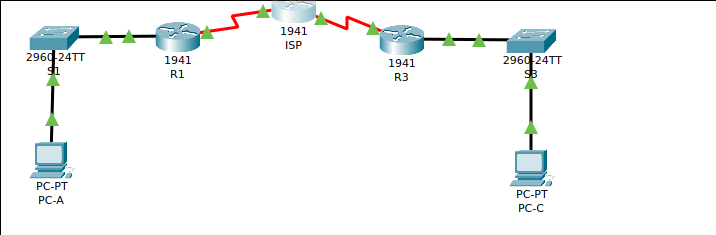
\includegraphics[width=.45\linewidth]{Figures/Topology.png}\par
\caption{Topology of the Network}\label{P1Top18}
\end{figure}


\noindent\mysubsection{2}{Initialize and reload the routers and switches}\\
I initialized the routers for the network, their configurations
can be seen in Fig.~\ref{P1Conf18R}\subref{P1Conf18R1} through
Fig.~\ref{P1Conf18R}\subref{P1Conf18R3} on Pg.~\pageref{P1Conf18R}


\begin{figure}[!hbt]\centering
\subfloat[Show ip int of R1]{\label{P1Conf18R1}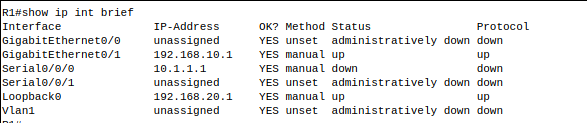
\includegraphics[width=.45\linewidth]{Figures/2020-03-24-114323_587x123_scrot.png}}\hfill
\subfloat[Show Ip Int of ISP]{\label{P1Conf18R2}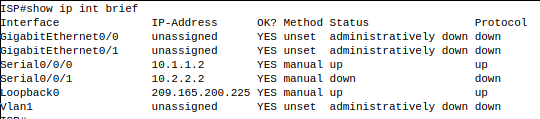
\includegraphics[width=.45\linewidth]{Figures/2020-03-24-114856_540x119_scrot.png}}\par
\subfloat[Show Ip int of R3]{\label{P1Conf18R3}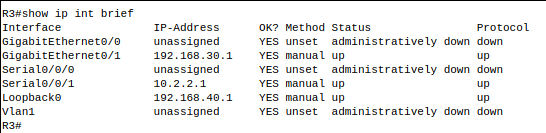
\includegraphics[width=.45\linewidth]{Figures/2020-03-24-115202_546x133_scrot.png}}\par
\caption{Configuring the Routers on the network}\label{P1Conf18R}
\end{figure}

\clearpage

I initialized the routers for the network, their configurations
can be seen in Fig.~\ref{P1Conf18S}\subref{P1Conf18S1a} through
Fig.~\ref{P1Conf18S}\subref{P1Conf18S3b} on Pg.~\pageref{P1Conf18S}


\begin{figure}[!hbt]\centering
\subfloat[Configuring S1]{\label{P1Conf18S1a}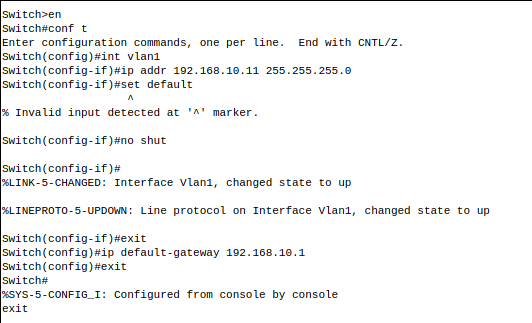
\includegraphics[width=.45\linewidth]{Figures/2020-03-24-115537_532x323_scrot.png}}\hfill
\subfloat[Show ip  int brief of S1]{\label{P1Conf18S1b}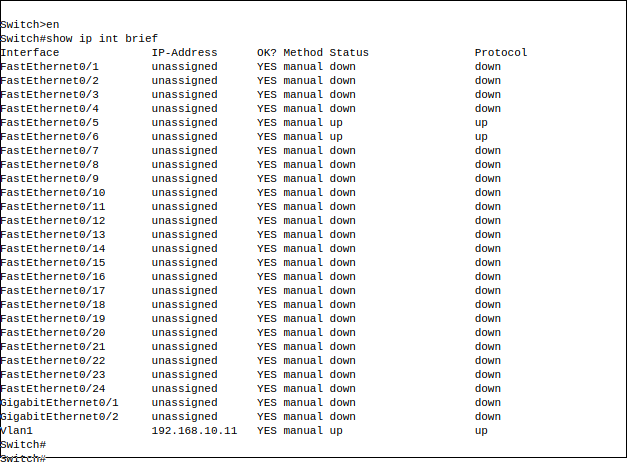
\includegraphics[width=.45\linewidth]{Figures/2020-03-24-115512_627x464_scrot.png}}\par
\subfloat[Configuring S3]{\label{P1Conf18S3a}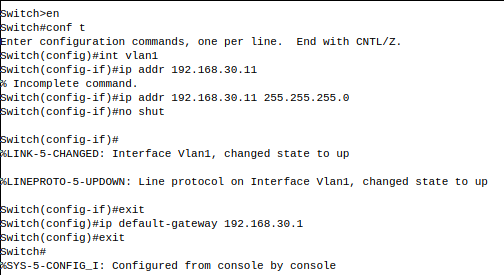
\includegraphics[width=.45\linewidth]{Figures/2020-03-24-115712_504x275_scrot.png}}\hfill
\subfloat[Show ip int brief of S3]{\label{P1Conf18S3b}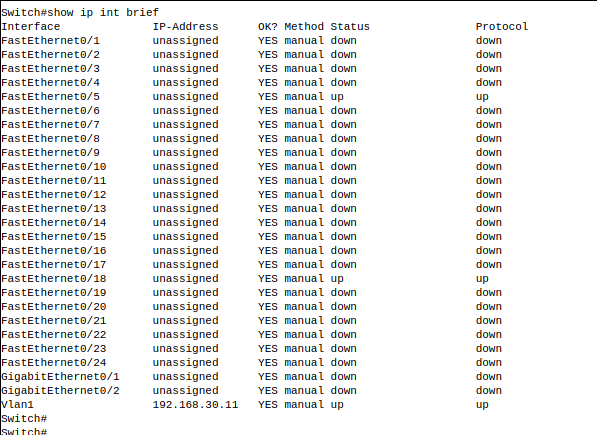
\includegraphics[width=.45\linewidth]{Figures/2020-03-24-115736_597x435_scrot.png}}\par
\caption{Configuring the switches on the network}\label{P1Conf18S}
\end{figure}


\clearpage

%===================================
\mysection{\textbf{Part 2: Configure Devices and Verify Connectivity }}

\mysubsection{1}{Configure IP addresses on PC-A and PC-C}\\
I configured the PCs for the network. See Fig.~\ref{P2Conf18PC} on
Pg.~\pageref{P2Conf18PC}.


\begin{figure}[!hbt]\centering
\subfloat[IP Configuration of PC-a]{\label{P2Conf18PCa}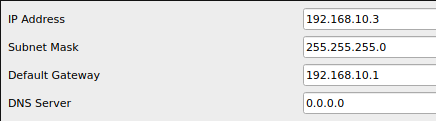
\includegraphics[width=.45\linewidth]{Figures/2020-03-24-115843_436x121_scrot.png}}\hfill
\subfloat[IP configuration of PC-C]{\label{P2Conf18PCb}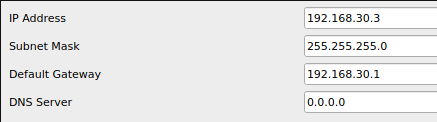
\includegraphics[width=.45\linewidth]{Figures/2020-03-24-115910_437x122_scrot.png}}\par 
\caption{IP configurations for the PCs of the network}\label{P2Conf18PC}
\end{figure}




\noindent\mysubsection{2}{Configure basic settings for the routers}\\
I configured the basic settings, and then copied the running config to the
starting config.


\begin{figure}[!hbt]\centering
\subfloat[Copy Show-run R1]{\label{P2Config18R1}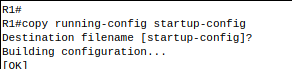
\includegraphics[width=.45\linewidth]{Figures/2020-03-24-121403_292x69_scrot.png}}\hfill
\subfloat[Copy Show-run ISP]{\label{P2Config18R2}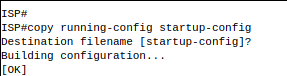
\includegraphics[width=.45\linewidth]{Figures/2020-03-24-121415_287x76_scrot.png}}\par 
\subfloat[CopyShow-run R3]{\label{P2Config18R3}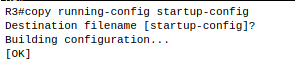
\includegraphics[width=.45\linewidth]{Figures/2020-03-24-121430_295x64_scrot.png}}
\caption{Basic configurations of the routers}\label{P2Config18R}
\end{figure}

\clearpage

\noindent\mysubsection{3}{Configure RIP routing on R1, ISP, and R3}\\
I Set the Routers on the network up for RIP V2. See Fig.~\ref{P2RipA18} on
Pg.~\pageref{P2RipA18}.
I then Verified the connections on each of the networks, running the commands
{\scriptsize{\verb$show ip protocols$}\normalsize} and
{\scriptsize{\verb$show ip route$}\normalsize}. See Fig.~\ref{P2RipB18} on
Pg.~\pageref{P2RipB18}.


\begin{figure}[!hbt]\centering
\subfloat[RipV2 setup on R1]{\label{P2RipA18R1}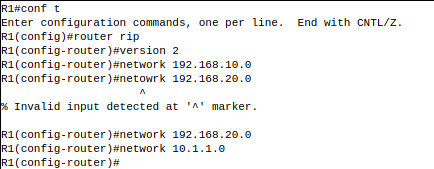
\includegraphics[width=.45\linewidth]{Figures/2020-03-24-121637_434x169_scrot.png}}\hfill
\subfloat[RipV2 setup on ISP]{\label{P2RipA18R2}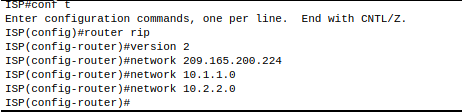
\includegraphics[width=.45\linewidth]{Figures/2020-03-24-121756_462x112_scrot.png}}\par 
\subfloat[RipV2 setup on R3]{\label{P2RipA18R3}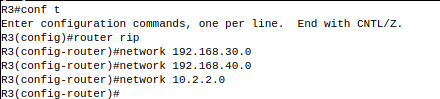
\includegraphics[width=.45\linewidth]{Figures/2020-03-24-122021_440x99_scrot.png}}
\caption{Configuring Rip V2 on the routers}
\label{P2RipA18}
\end{figure}


\begin{figure}[!hbt]\centering
\subfloat[show ip protocols on R1]{\label{P2RipB18r1}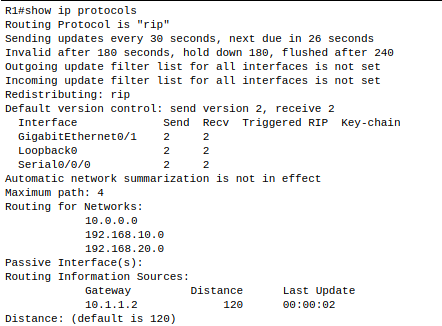
\includegraphics[width=.45\linewidth]{Figures/2020-03-24-123450_442x326_scrot.png}}\hfill
\subfloat[show ip route on R1]{\label{P2RipB18r2}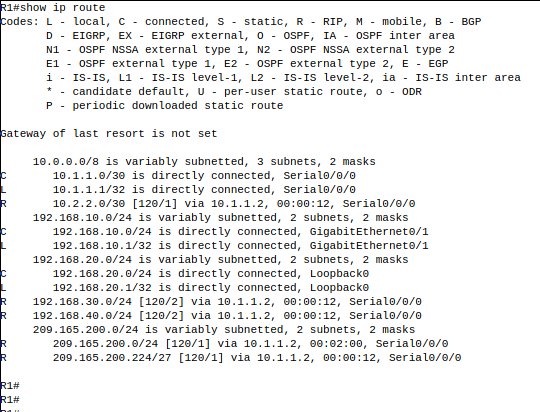
\includegraphics[width=.45\linewidth]{Figures/2020-03-24-123546_540x412_scrot.png}}\par
\subfloat[show ip protocols on ISP]{\label{P2RipB18r3}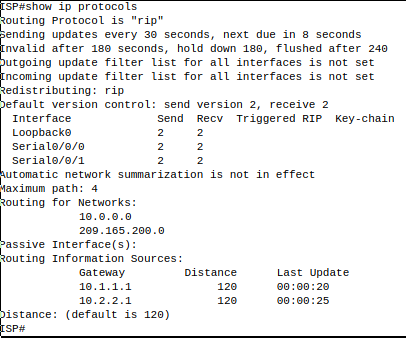
\includegraphics[width=.45\linewidth]{Figures/2020-03-24-123500_406x338_scrot.png}}\hfill
\subfloat[show ip route on ISP]{\label{P2RipB18r4}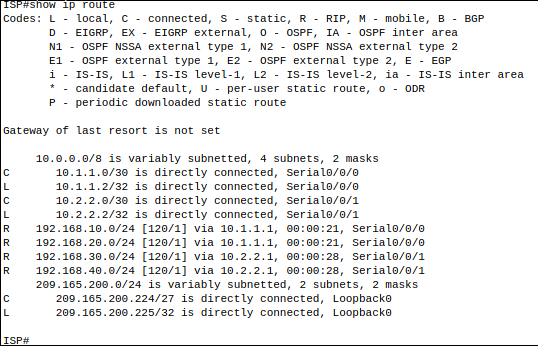
\includegraphics[width=.45\linewidth]{Figures/2020-03-24-123606_538x346_scrot.png}}\par
\subfloat[show ip protocols on R3]{\label{P2RipB18r5}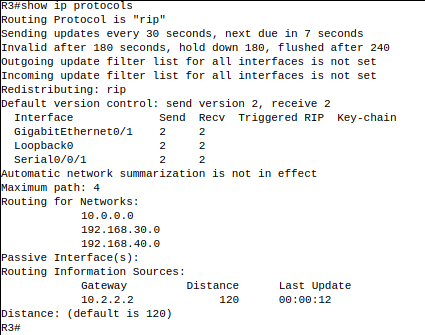
\includegraphics[width=.45\linewidth]{Figures/2020-03-24-123508_425x335_scrot.png}}\hfill
\subfloat[show ip route on R3]{\label{P2RipB18r6}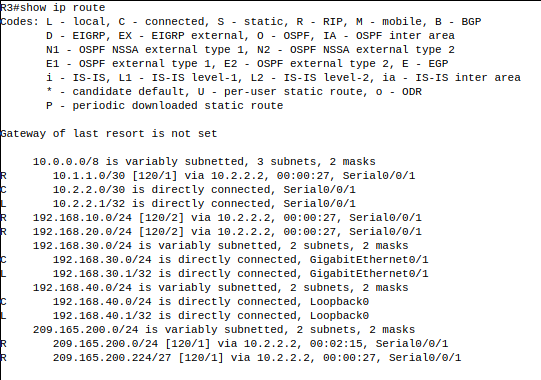
\includegraphics[width=.45\linewidth]{Figures/2020-03-24-123624_541x380_scrot.png}}\par
\caption{Verifying RIPv2 on the routers}
\label{P2RipB18}
\end{figure}

\clearpage

\noindent\mysubsection{4}{Verify connectivity between Devices}\\
\noindent{\bf{a.}}\\
The pings from PC-A to PC-C and from PC-A to the loopback on R3 were both
successful. See
Fig.~\ref{P2Verify18}\subref{P2Verify18P1} on Pg.~\pageref{P2Verify18}.

\noindent{\bf{b.}}\\
The pings from R1 to PC-C and to the loopback interface on R3 were both successful. See
Fig.~\ref{P2Verify18}\subref{P2Verify18P2} on Pg.~\pageref{P2Verify18}.

\noindent{\bf{c.}}\\
The pings from PC-C to PC-A and the loopback interface of R1 were both
successful. See
Fig.~\ref{P2Verify18}\subref{P2Verify18P3} on Pg.~\pageref{P2Verify18}.

\noindent{\bf{d.}}\\
The pings from R3 to PC-A and the loopback interface on R1 were both successful. See
Fig.~\ref{P2Verify18}\subref{P2Verify18P4} on Pg.~\pageref{P2Verify18}.

\begin{figure}[!hbt]\centering
\subfloat[PC-A to PCC and R3 loopback]{\label{P2Verify18P1}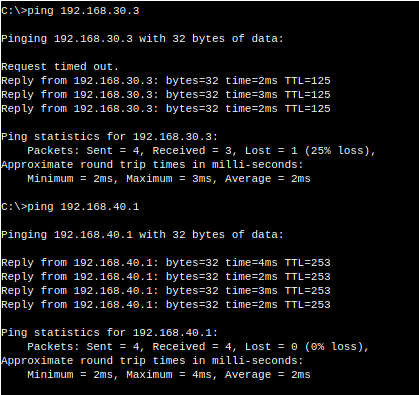
\includegraphics[width=.45\linewidth]{Figures/2020-03-24-123753_419x395_scrot.png}}\hfill
\subfloat[R1 to PC-C and R3 loopback]{\label{P2Verify18P2}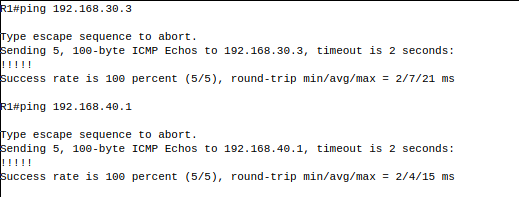
\includegraphics[width=.45\linewidth]{Figures/2020-03-24-123854_519x197_scrot.png}}\par
\subfloat[PC-C to PC-A and R1 loopback]{\label{P2Verify18P3}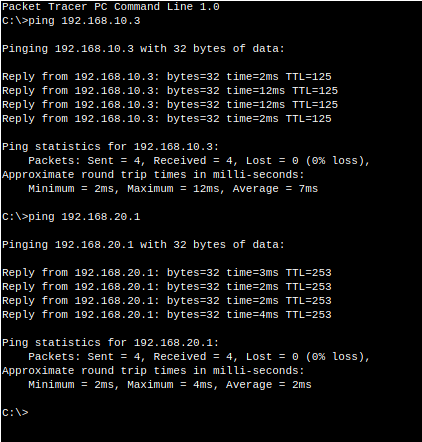
\includegraphics[width=.45\linewidth]{Figures/2020-03-24-124019_422x442_scrot.png}}\hfill
\subfloat[R3 to PC-A and R1 loopback]{\label{P2Verify18P4}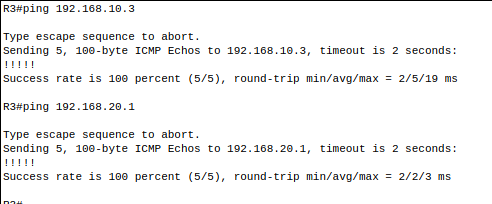
\includegraphics[width=.45\linewidth]{Figures/2020-03-24-124026_492x204_scrot.png}}\par
\caption{Verifying connection on the network}\label{P2Verify18}
\end{figure}


\clearpage

%===================================
\mysection{\textbf{Part 3: Configure and Verify Standard Numbered and Named ACLs}}

\mysubsection{1}{Configure a numbered standard ACL}\\
What wildcart mask would you use to allow all hosts on the 192.168.10.0/24
network to access the 192.168.30.0/24 network?\\
I would use the 0.0.0.255 wildcard to allow any host from the
192.168.10.anything.


Following Cisco's recommended best practices, on which router would you place
this ACL?\\
router 3, becuase is closest to the network we want to restrict access to.

On which interface would you place this ACL? In what direction would you apply it?\\

I would place it on G0/1. And I would make it OUtbound.

\noindent{\bf{a. And b.}}
I configured it according to the file and then I applied the ACL (Fig.~\ref{P3NuACL18}\subref{P3NuACL18a})

\noindent{\bf{c.}}
{\bf{1}}
I verified the ACL was in place with
{\scriptsize{\verb$show access-lists$}\normalsize}
(Fig.~\ref{P3NuACL18}\subref{P3NuACL18b}).

{\bf{2}}
then ran
{\scriptsize{\verb$show ip int g0/1$}\normalsize}
(Fig.~\ref{P3NuACL18}\subref{P3NuACL18c}).

{\bf{3}} PC-A succssesfully pinging PC-C (Fig.~\ref{P3NuACL18}\subref{P3NuACL18d}).
{\bf{4}} And then successfully pinging PC-C with an extended ping from the loopback address on R1
(Fig.~\ref{P3NuACL18}\subref{P3NuACL18e})


\begin{figure}[!hbt]\centering
\subfloat[Configuring and Applying the ACL to
R3]{\label{P3NuACL18a}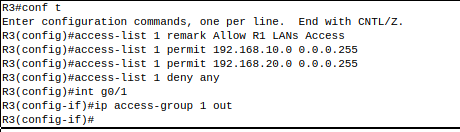
\includegraphics[width=.45\linewidth]{Figures/2020-03-24-124409_460x132_scrot.png}}\hfill
\subfloat[Show access-lists on
R3]{\label{P3NuACL18b}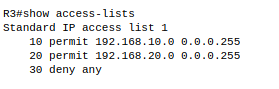
\includegraphics[width=.45\linewidth]{Figures/2020-03-24-124424_279x89_scrot.png}}\par
\subfloat[Show ip int G0/1 on
R3]{\label{P3NuACL18c}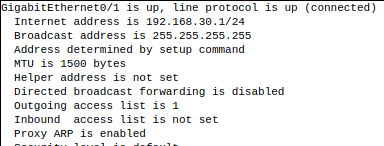
\includegraphics[width=.45\linewidth]{Figures/2020-03-24-124439_384x146_scrot.png}}\par
\subfloat[PC-A pinging
PC-C]{\label{P3NuACL18d}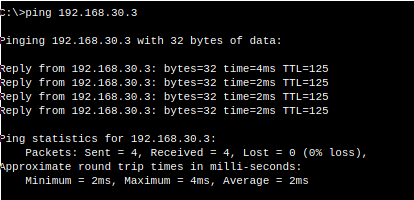
\includegraphics[width=.45\linewidth]{Figures/2020-03-24-124534_414x200_scrot.png}}\hfill
\subfloat[R3 loopback pinging
PC-C]{\label{P3NuACL18e}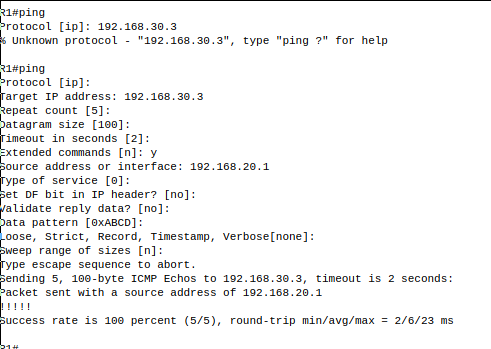
\includegraphics[width=.45\linewidth]{Figures/2020-03-24-124754_491x349_scrot.png}}\par
\caption{Configuring a Named ACL on R3}\label{P3NuACL18}
\end{figure}

\clearpage

\noindent\mysubsection{2}{Configure a named standard ACL}\\
Following Cisco's best practices, on which router would you place this ACL?\\
I would place it on R1.


On which interface would you place this ACL? In what direction would you apply
it?\\
I would place it on G0/1 as an outbound policy.


\noindent{\bf{a. And b.}}
I configured it according to the file and then I applied the ACL (Fig.~\ref{P3NaACL18}\subref{P3NaACL18a})

\noindent{\bf{c.}}
{\bf{1}}
I verified the ACL was in place with
{\scriptsize{\verb$show access-lists$}\normalsize}
(Fig.~\ref{P3NaACL18}\subref{P3NaACL18b}).

{\bf{2}}
then ran
{\scriptsize{\verb$show ip int g0/1$}\normalsize}
(Fig.~\ref{P3NaACL18}\subref{P3NaACL18c}).

{\bf{3}} PC-C succssesfully pinging PC-A (Fig.~\ref{P3NaACL18}\subref{P3NaACL18d}).
{\bf{4}} And then unsuccessfully pinging PC-A with an extended ping from the
G0/1 address on R3 (Fig.~\ref{P3NaACL18}\subref{P3NaACL18e})
{\bf{5}} Successfully pinging PC-A with an Extended ping from the loopback
address on R3 (Fig.~\ref{P3NaACL18}\subref{P3NaACL18f}).


\begin{figure}[!hbt]\centering
\subfloat[Configuring and applying the ACL on R1]{\label{P3NaACL18a}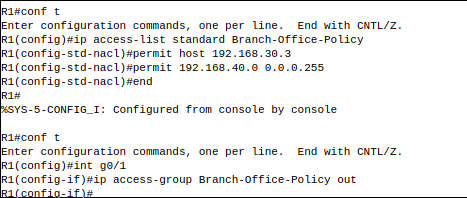
\includegraphics[width=.45\linewidth]{Figures/2020-03-24-125038_467x198_scrot.png}}\hfill
\subfloat[show access-lists on R1]{\label{P3NaACL18b}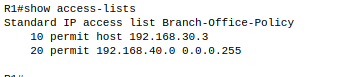
\includegraphics[width=.45\linewidth]{Figures/2020-03-24-125102_342x77_scrot.png}}\par
\subfloat[show ip int g0/1 on R1]{\label{P3NaACL18c}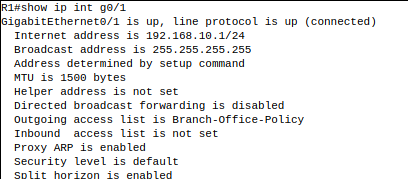
\includegraphics[width=.45\linewidth]{Figures/2020-03-24-125123_408x179_scrot.png}}\hfill
\subfloat[PC-C pinging PC-A]{\label{P3NaACL18d}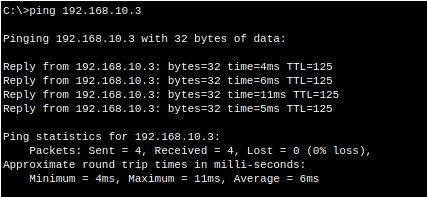
\includegraphics[width=.45\linewidth]{Figures/2020-03-24-125201_427x197_scrot.png}}\par
\subfloat[Pinging PC-A from G0/1 on R3]{\label{P3NaACL18e}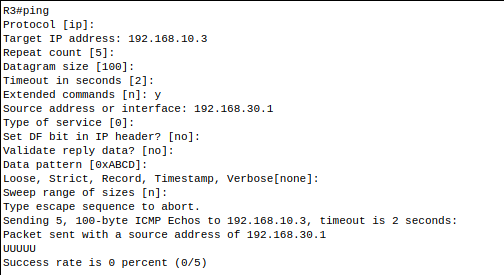
\includegraphics[width=.45\linewidth]{Figures/2020-03-24-125323_504x275_scrot.png}}\hfill
\subfloat[Pinging PC-A from loopback0 on R3]{\label{P3NaACL18f}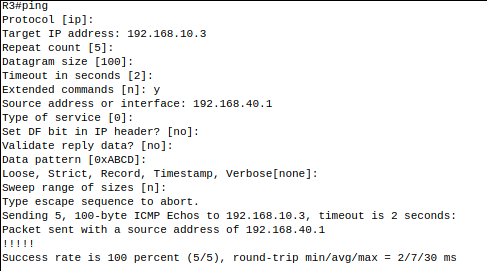
\includegraphics[width=.45\linewidth]{Figures/2020-03-24-125439_487x271_scrot.png}}\par
\caption{Configuring and verifying a named ACL on R1}\label{P3NaACL18}
\end{figure}

\clearpage

%===================================
\mysection{\textbf{Part 4: Modify a Standard ACL}}

\mysubsection{1}{Modify a named standard ACL}\\
{\bf{a}}\\
I ran {\scriptsize{\verb$show access-lists$}\normalsize} on
R1 (Fig.~\ref{P4Mod18}\subref{P4Mod18a}). 


{\bf{b}}\\
I added two aditional Policies to
Branch-Office-Policy (Fig.~\ref{P4Mod18}\subref{P4Mod18b}).


{\bf{c}}\\
I ran show access-lists again to show the newly configured
access-list (Fig.~\ref{P4Mod18}\subref{P4Mod18c}).

{\bf{1}}\\
No, I don't have to reapply it because I only updated the policy that had
already been placed on G0/1 on R1. Seen from the 
{\scriptsize{\verb$show ip int g0/1$}\normalsize}
output(Fig.~\ref{P4Mod18}\subref{P4Mod18d}).


{\bf{2}}\\
From the ISP router I ran an extended ping from the loopback 0 address, to
PC-A's IP address successfully (Fig.~\ref{P4Mod18}\subref{P4Mod18e}).


\begin{figure}[!hbt]\centering
\subfloat[show access-lists before modifying]{\label{P4Mod18a}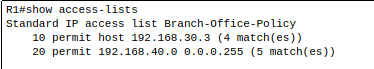
\includegraphics[width=.45\linewidth]{Figures/2020-03-24-125532_374x69_scrot.png}}\hfill
\subfloat[modifying ACL on R1]{\label{P4Mod18b}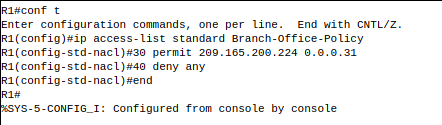
\includegraphics[width=.45\linewidth]{Figures/2020-03-24-125648_442x125_scrot.png}}\par
\subfloat[show access-lists after modification]{\label{P4Mod18c}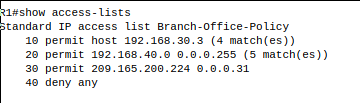
\includegraphics[width=.45\linewidth]{Figures/2020-03-24-125706_360x103_scrot.png}}\par
\subfloat[show ip int g0/1 after modification]{\label{P4Mod18d}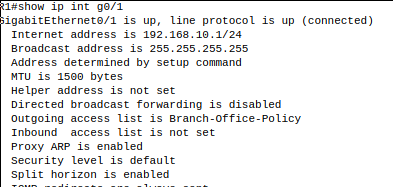
\includegraphics[width=.45\linewidth]{Figures/2020-03-24-125802_393x187_scrot.png}}\hfill
\subfloat[Pinging PC-A from loopback 0 of ISP]{\label{P4Mod18e}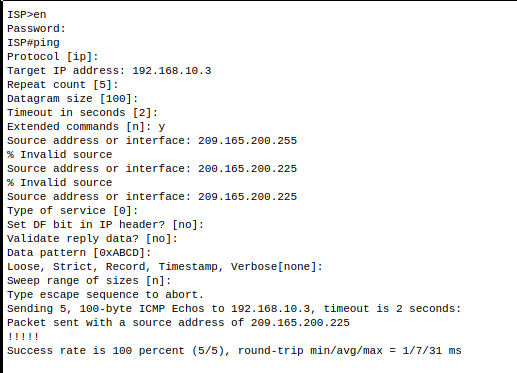
\includegraphics[width=.45\linewidth]{Figures/2020-03-24-130034_517x373_scrot.png}}\par
\caption{Modifying a named access-list}\label{P4Mod18}
\end{figure}

\clearpage

%===================================
\mysection{\textbf{Reflection}}

\mysubsection{1}{As you can see, standard ACLs are very powerful and work quite
well. Why would you ever have the need for using extended ACLs?}\\
Extended ACLs give the extra ability to control not just the host coming into
the network, but the host it is trying to reach. Also, gives the ability to
select based upon ports and protocols.

\noindent\mysubsection{2}{Typically more typing is required when using a named
ACL as opposed to a numbered ACL. Why would you choose named ACLs over
numbered?}\\
It would gives a lesser ability to accidentally choose the wrong name to
apply, because it has a name instead of a number. It also has the ability to
reduce the need for remarks on the name of it.

%===================================

\end{document}
